\begin{document}

\def\title{Homework 6}
% \config{hwnum}{2}
% \config{homework-due}{02/0/2019 23:59}
% \config{grades-due}{02/XX/2019 23:59}

\newcommand{\qitem}{\qpart\item}

\renewcommand{\labelenumi}{(\alph{enumi})} % change default enum format to (a)
\renewcommand{\theenumi}{(\alph{enumi})} % fix reference format accordingly.
\renewcommand{\labelenumii}{\roman{enumii}.} % second level labels.
\renewcommand{\theenumii}{\roman{enumii}.}

\maketitle
% \vspace{0.5em}
% {\textbf{Due date:} 2/8/19, at 23:59. Please \LaTeX of handwrite your homework solution and submit an electronic version on Gradescope.}

% {\textbf{Self-grades due date:} 2/XX/19, at 23:59.}

% {\parindent 0pt
% \begin{tabular}[t]{l}
% EECS 127 / EE 227AT \\
% G. Ranade, A. Bayen
% \end{tabular}  \hfill 2/1/19\vskip 0.2in }

% \parindent 0pt
% \parskip 8pt

% \begin{center}
% \large\bf Homework Assignment \#2
% \end{center}

% \bigskip

\noindent
{\bf Release date:} 10/10/19.\\
{\bf Due date:}  10/17/19, 23:00 (11 pm). Please \LaTeX{} or handwrite your homework solution and submit an electronic version. 

\textbf{Submission Format} \\
Your homework submission should consist of a single PDF file that contains all of your answers (any handwritten answers should be scanned) as well as your IPython notebook saved as a PDF.
			
If you do not attach a PDF ``printout'' of your IPython notebook, you will not receive credit for problems that involve coding. Make sure that your results and your plots are visible. Assign the IPython printout to the correct problem(s) on Gradescope.

\begin{qunlist}
\qns{Convexity of Sets and Functions}\\
In this problem we will determine if a set/function is a convex set/function. State reasoning for your answer and unless required, don't prove the properties for convexity as covered in class for each question. Although, doing it for your own practice will help you better prepare for similar questions in midterm/final.
\begin{enumerate}
\item
For the sets given below, determine if it is a convex set or not with proper justification for your answer.
\begin{enumerate}
    \item
    The empty set $\phi$
    \item
    A singleton set $\{x_0\}$
    \item
    $\mathbb{R}^n$
    \item
    $\mathcal{P} = \{(x_1,x_2)$, where $x_1$ is the date (1-31) and $x_2$ is the month (1-12) corresponding to the date of birth of EECS 127/227A students$\}$
    \item
    $\mathcal{P} = \{z : z = (1-t)\vec{a} + t\vec{b}$, where $a$ and $b$ are two vectors with same dimension as $z$ and $t\in [0,1]$\}
    \item
    $\mathcal{P} = \{z : \vec{a}\tran z = b, a \neq 0\}$
    \item
    $\mathcal{P} = \{z : \vec{a}\tran z \leq b, a \neq 0\}$
    \item
    $\mathcal{P} = \{z : \|z - \vec{z_0}\|_2 \eq \epsilon$\}
    \item
    $\mathcal{P} = \{z : \|z - \vec{z_0}\|_2 \leq \epsilon$\}
    \item
    $\mathcal{P}$ = epigraph($f$) = $\{(z,t) : z\in domain(f)$ and $t \geq f(z)\}$, where $f$ is a convex function
    \item
    $\mathcal{P} = Q\bigcap R$, where $Q$ and $R$ are convex sets
    \item
    $\mathcal{P}$  = Minkowski sum of sets $Q$ and $R$, where $Q$ and $R$ are convex sets, where Minkowski sum of two sets $Q$ and $R$ is defined as $Q + R =\{q +r \,|\,q \in Q,\ r \in R\}$.
    \item
    $\mathcal{P} = \{(x_1,x_2): (x_1 \geq x_2-1 \;\;\text{and}\;\; x_2 \geq 0) \;\;\text{OR}\;\; (x_1 \leq x_2-1 \;\;\text{and}\;\; x_2 \leq 0)\}$
\end{enumerate}
\sol{
    \item $g(x_1,x_2) = \dfrac{x_1^2}{4} + \dfrac{x_2^2}{9}$



    }
\item
For the functions given below, determine if it is a convex function or not with proper justification for your answer.
\begin{enumerate}
    \item
    $f(x) = a\tran \vec{x} + b$
    \item
    $f(x) = \cos(x), x\in [\frac{\pi}{2},\frac{3\pi}{2}]$
    \item
    $f(\vec{x}) = \vec{x}\tran Q\vec{x} + a\tran \vec{x} + b$, where $Q$ is Positive Semi-definite
    \item
    $\sum_{i}w_if_i(x)$, $w_i \in \mathbb{R}$ and each $f_i$ convex
    \item
    $f(A\vec{x}+b)$, where $f$ is a convex function
    \item 
    $f(x) = \max_i f_i(x)$, where $f_i$ are convex functions
    \item
    $g(f(x))$, where f(x) is convex and g(x) is convex and non-decreasing
    \item
    $f(x)$ a function whose epigraph is a convex set
\end{enumerate}
\sol{
    \item Show that the following inequalities hold for any vector $x \in \Real{n}$:
\[
% \|x\|_\infty \le \|x\|_1 \le n \|x\|_\infty \\
% \|x\|_2 \le \|x\|_1 \le \sqrt{n} \|x\|_2 \\
% \|x\|_\infty \le \|x\|_2 \le\sqrt{n}\|x\|_\infty \\
\frac{1}{\sqrt{n}}\|x\|_2 \leq \|x\|_\infty \leq  \|x\|_2 \leq \|x\|_1 \leq \sqrt{n} \|x\|_2 \le n\|x\|_\infty.
\]

\textit{Hint:} For $\|x\|_1\leq \sqrt{n}\|x\|_2$, how might you express $\|x\|_1$ as the dot product of two vectors? Can you then use the Cauchy-Schwarz inequality to bound this dot product?
    }
\item
For all the sets given in the following question, find the convex hull of the set.
\begin{enumerate}
    \item 
    $\mathcal{P} = \{(1,1),(2,3),(5,2)\}$
    \item
    $\mathcal{P} = \{x: x = sin(\theta), \theta \in \mathbb{R}\}$
    \item$\mathcal{P} = \{z : \|z - \vec{z_0}\|_2 \eq \epsilon$\}
    \item
    \textit{Bonus (This question will not be graded):} Assume the earth is round, and does not have any atmosphere. It has mountains, rivers, UC Berkeley and all the non-living things, and only \textquotedblleft Oski the Bear\textquotedblright shaped mammals roaming around. Considering the set of points covering all these system, what is the convex hull of the set?\\
    \textit{Hint: Think geometrically what convex hull represents and how you will obtain that geometrical shape for the planet mentioned in the question.}
    \\[1cm]
\end{enumerate}
\sol{
\item $g(x) = \sin(x_1^2) \log (x_3 - x_2)$ where $x_i$ are scalars and $x_3 - x_2 > 0$.
}
\item
Following are the candid shots collected from secret sources, where the EECS 127/227A course staff is shown frustrated with their laptop charger wires. Determine if the function corresponding to the curve formed by their laptop charger wire is convex or not with proper justification.
 \begin{figure}[H]
     \centering
     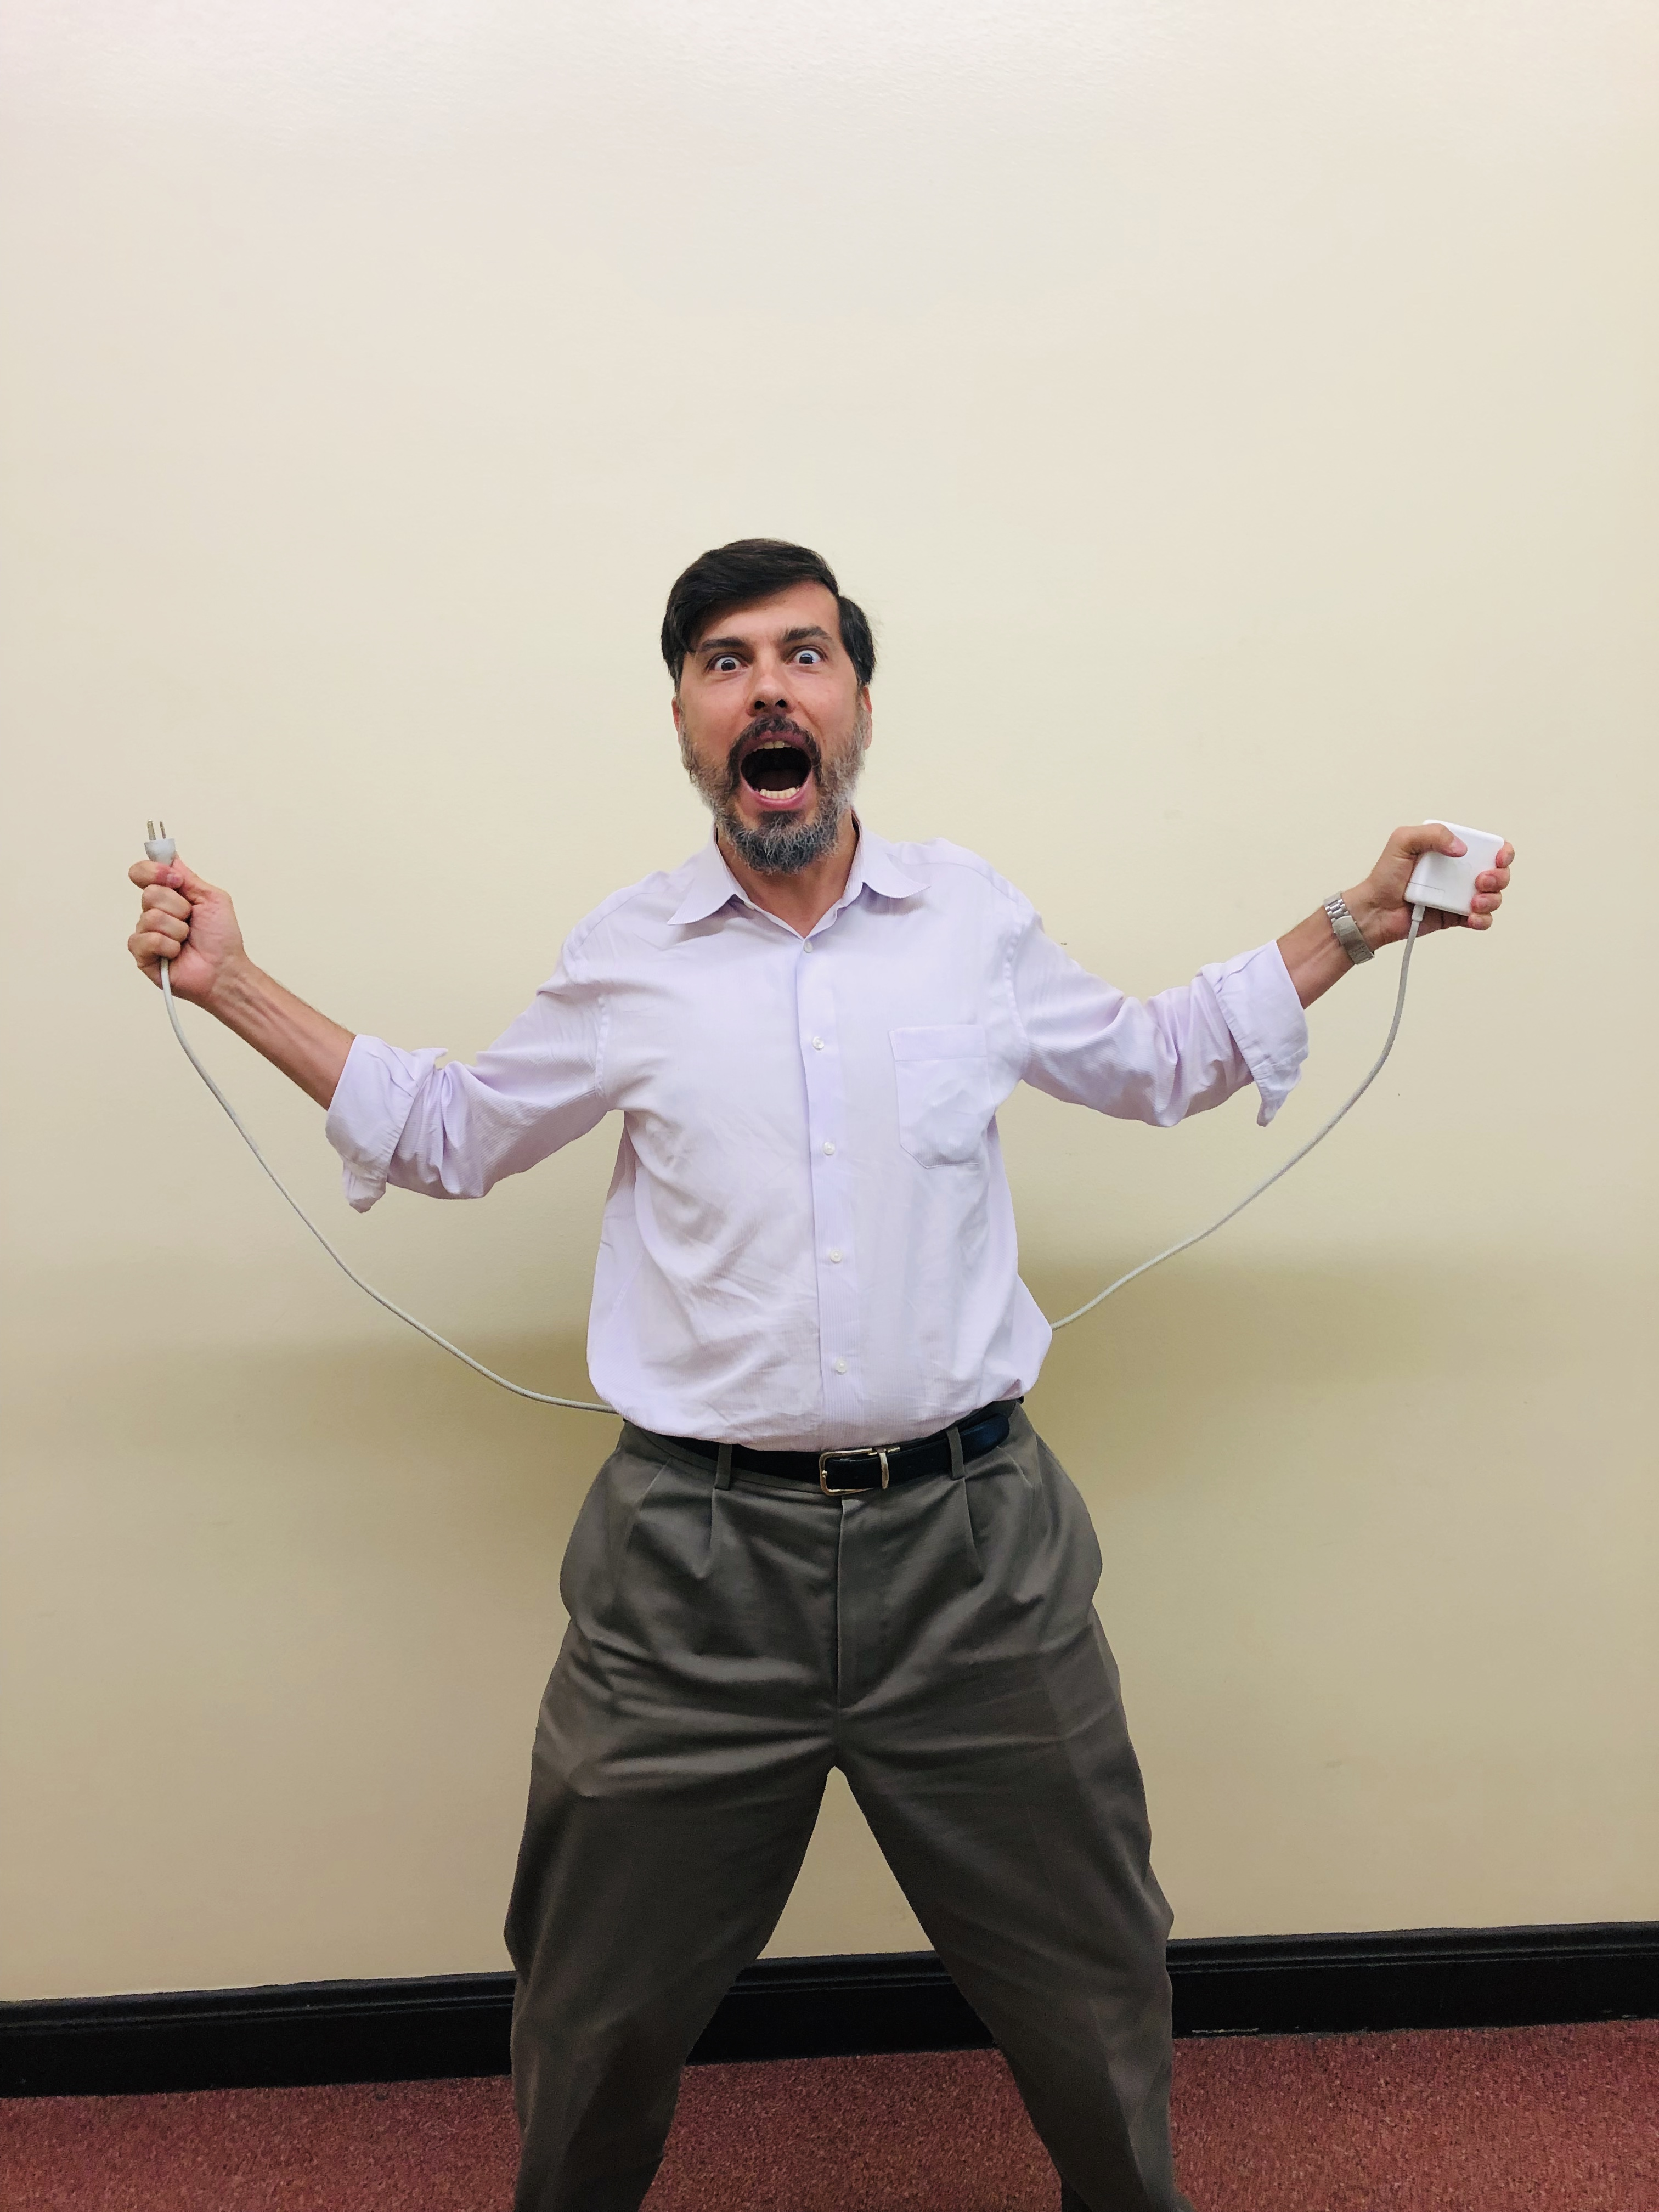
\includegraphics[width=0.45\textwidth]{figures/ab.jpg}
     \caption{Prof. Bayen's laptop wire curve}
 \end{figure}
 \begin{figure}[H]
  \centering
  \begin{minipage}[b]{0.45\textwidth}
    \includegraphics[height=9cm]{figures/catenary.png}
    \caption{GSI Theo's laptop wire curve}
  \end{minipage}
  \hfill
  \begin{minipage}[b]{0.45\textwidth}
    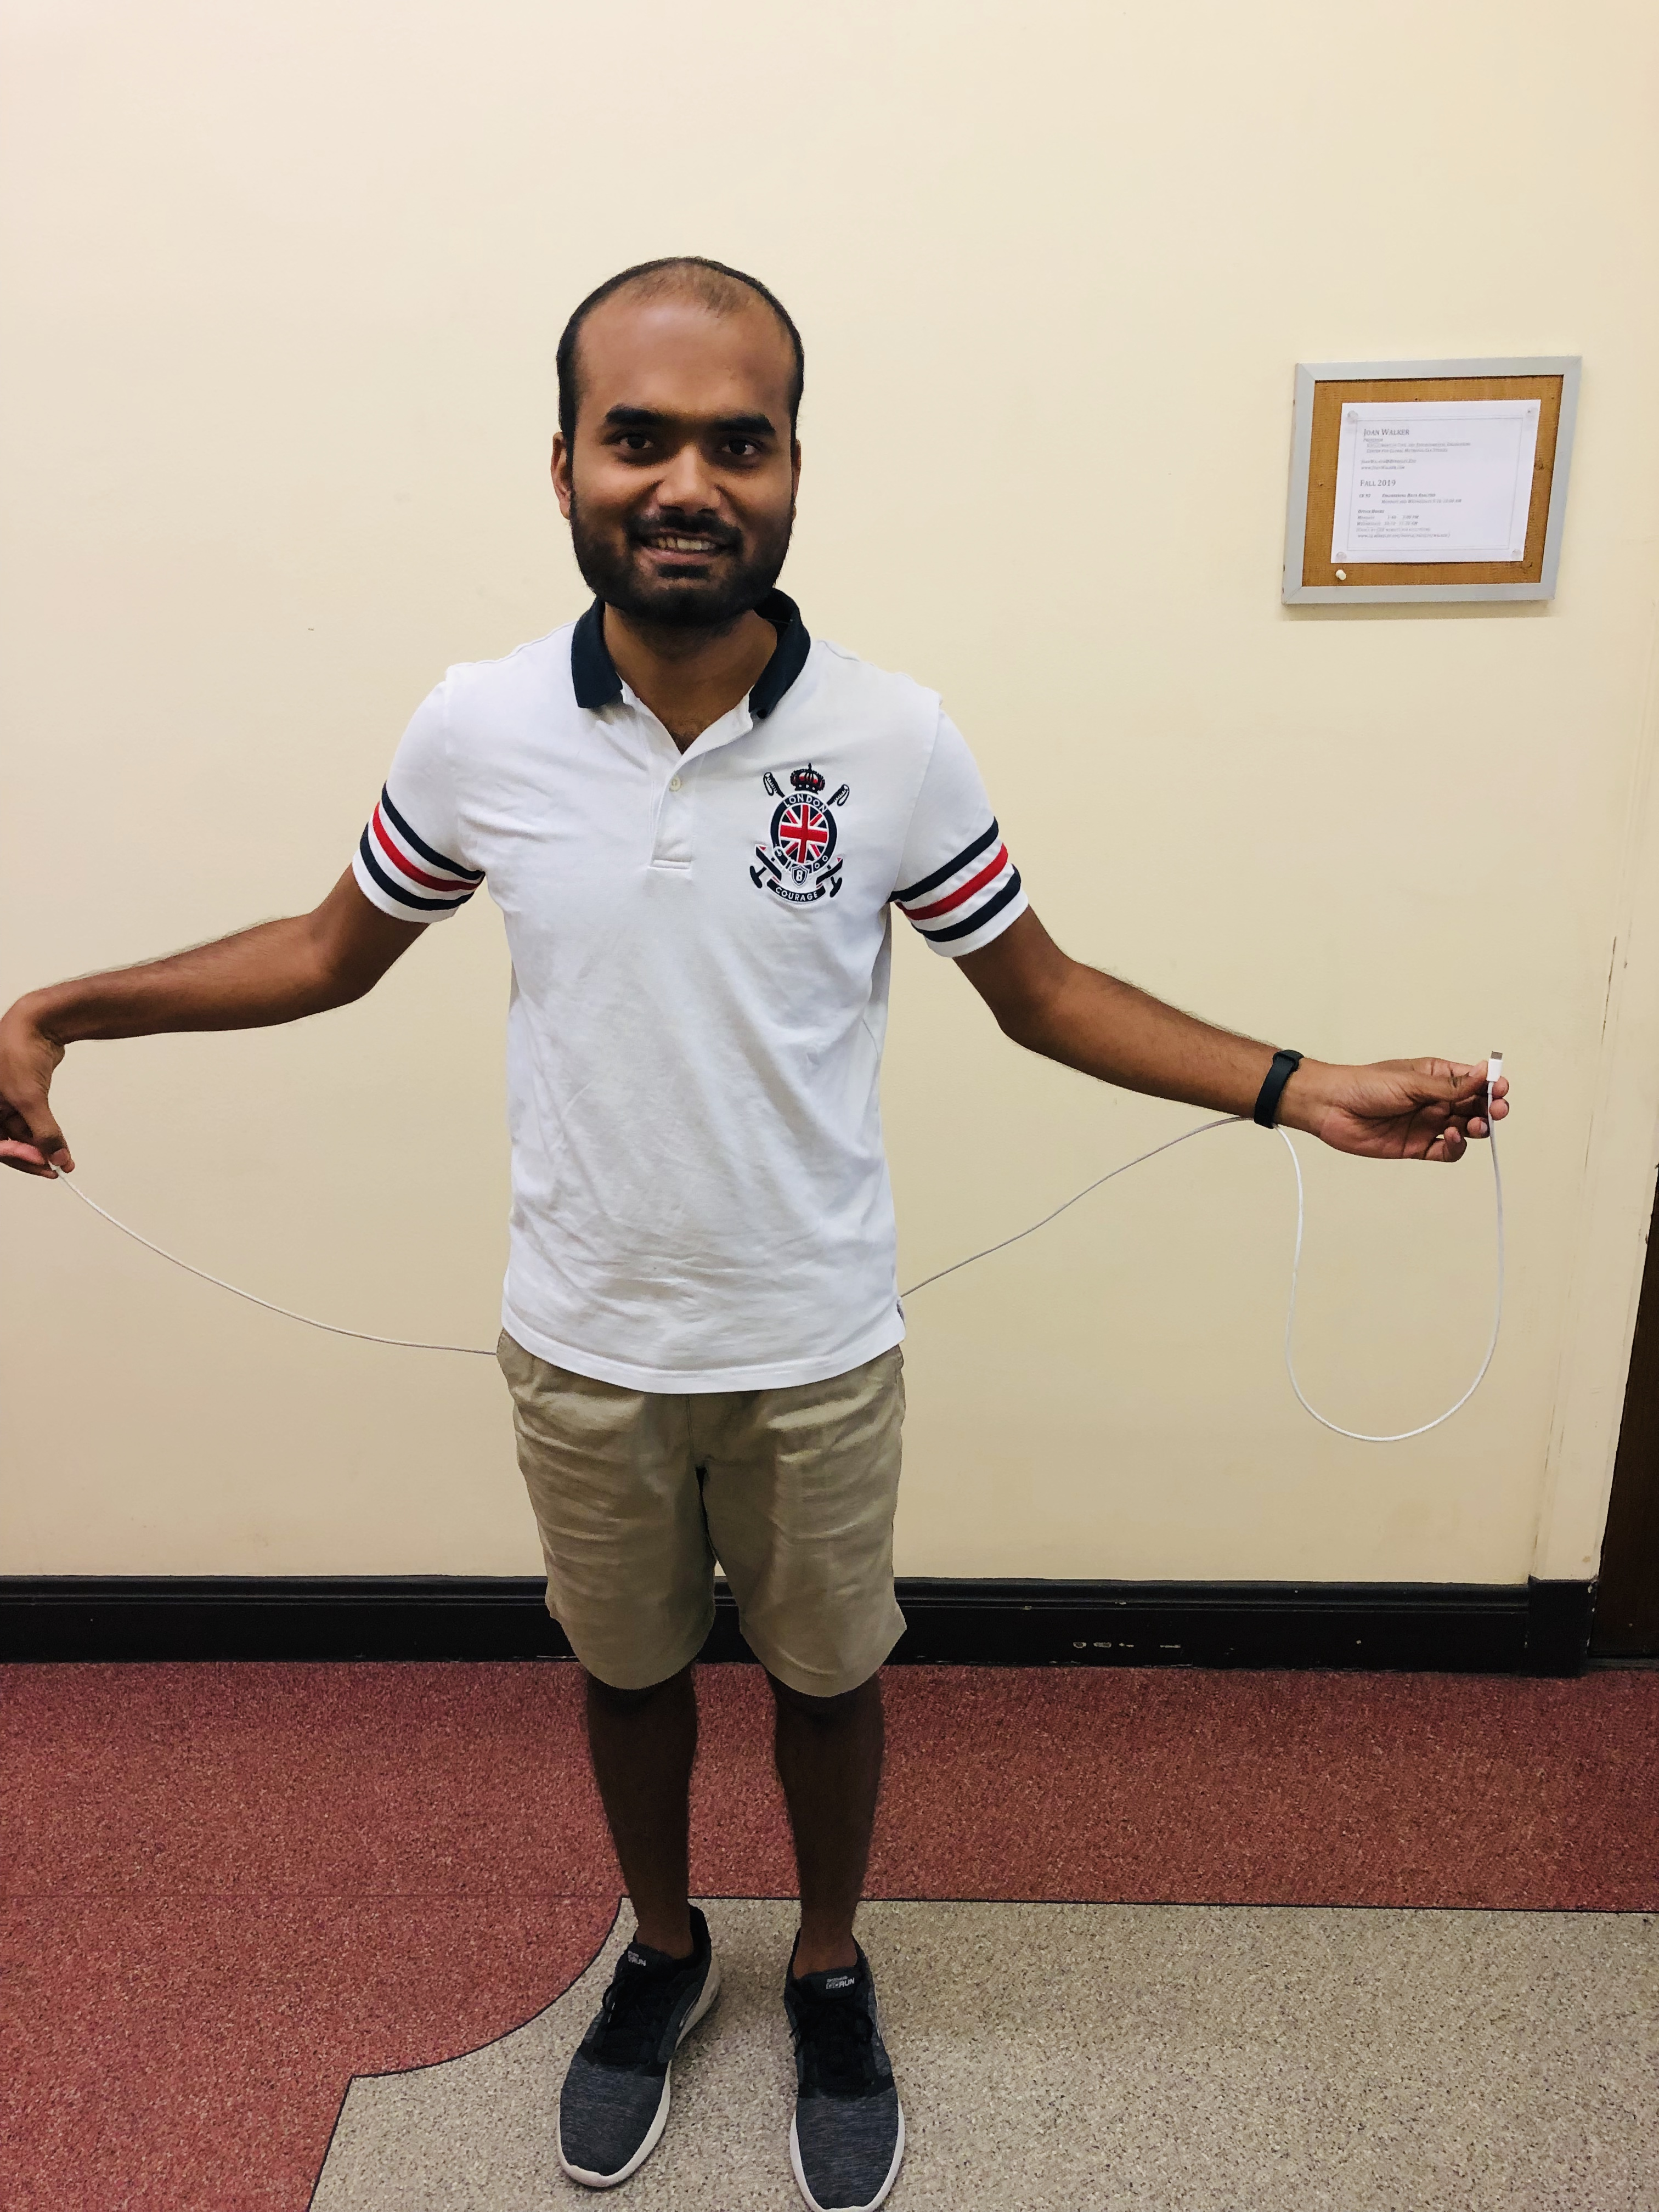
\includegraphics[height=9cm]{figures/hpd.jpg}
    \caption{GSI Hari's laptop wire curve}
  \end{minipage}
\end{figure}
\begin{figure}[H]
  \centering
  \begin{minipage}[b]{0.45\textwidth}
    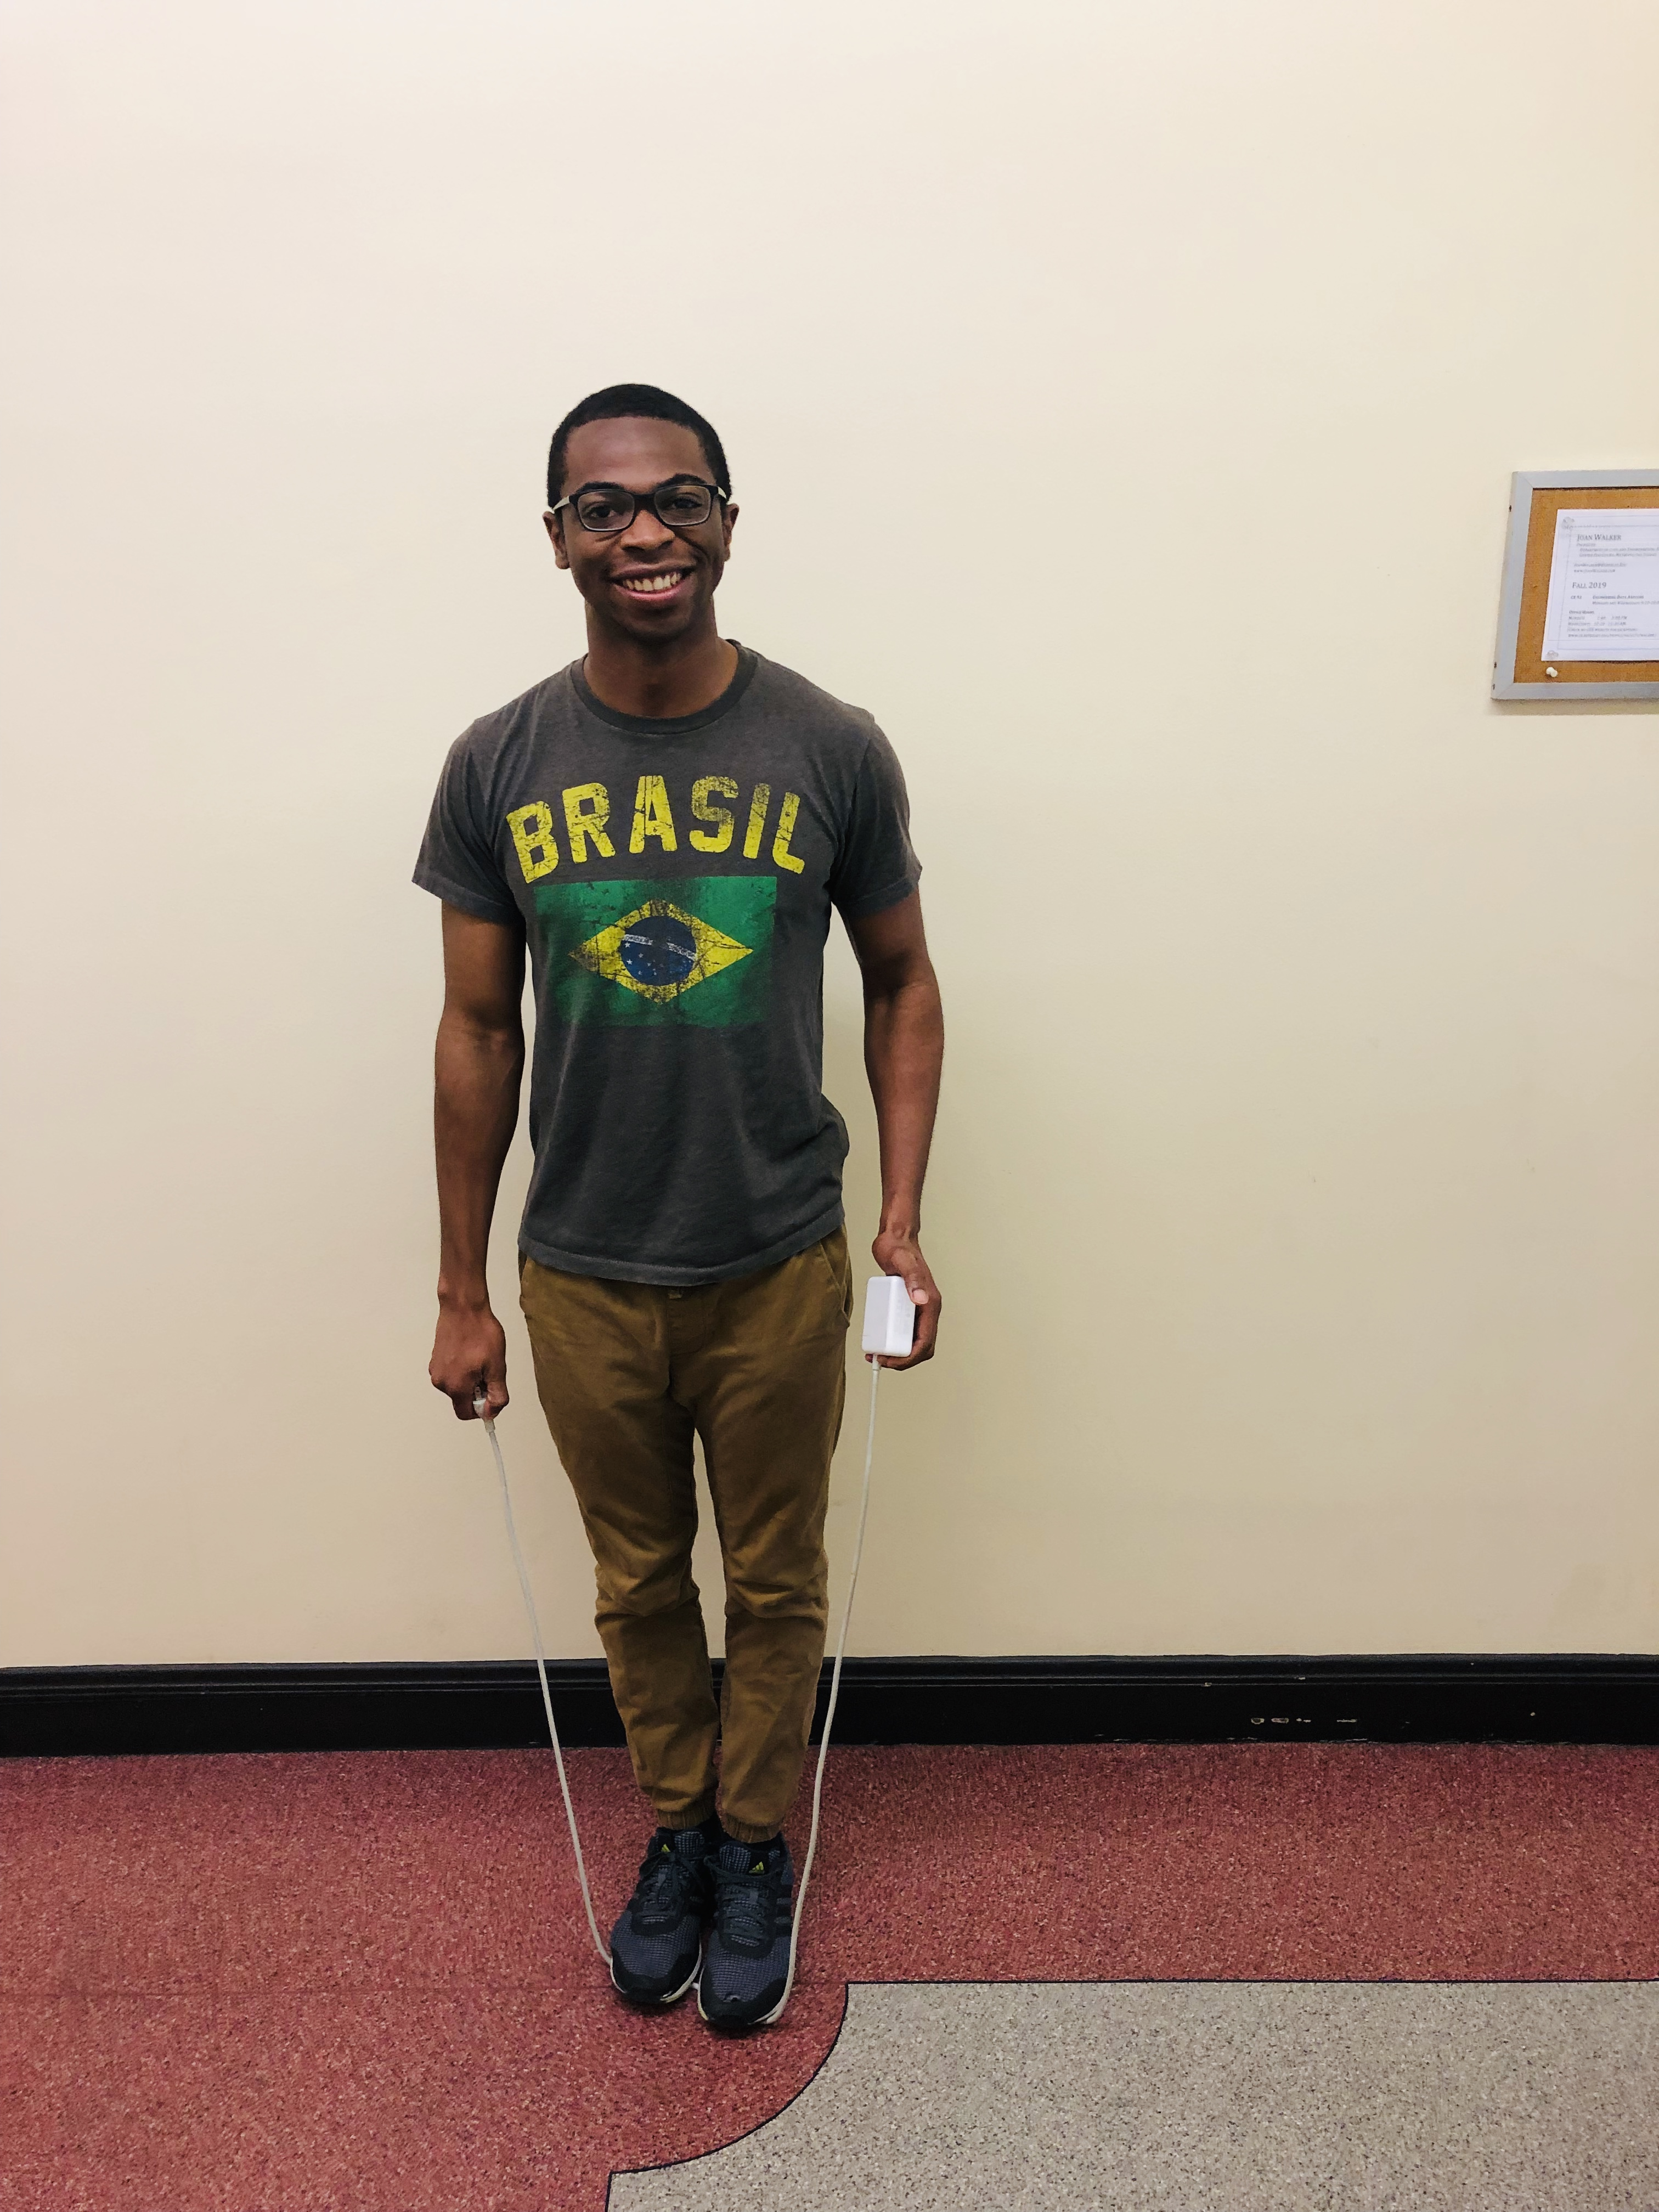
\includegraphics[height=9cm]{figures/oa.jpg}
    \caption{GSI Oladapo's laptop wire curve}
  \end{minipage}
  \hfill
  \begin{minipage}[b]{0.45\textwidth}
    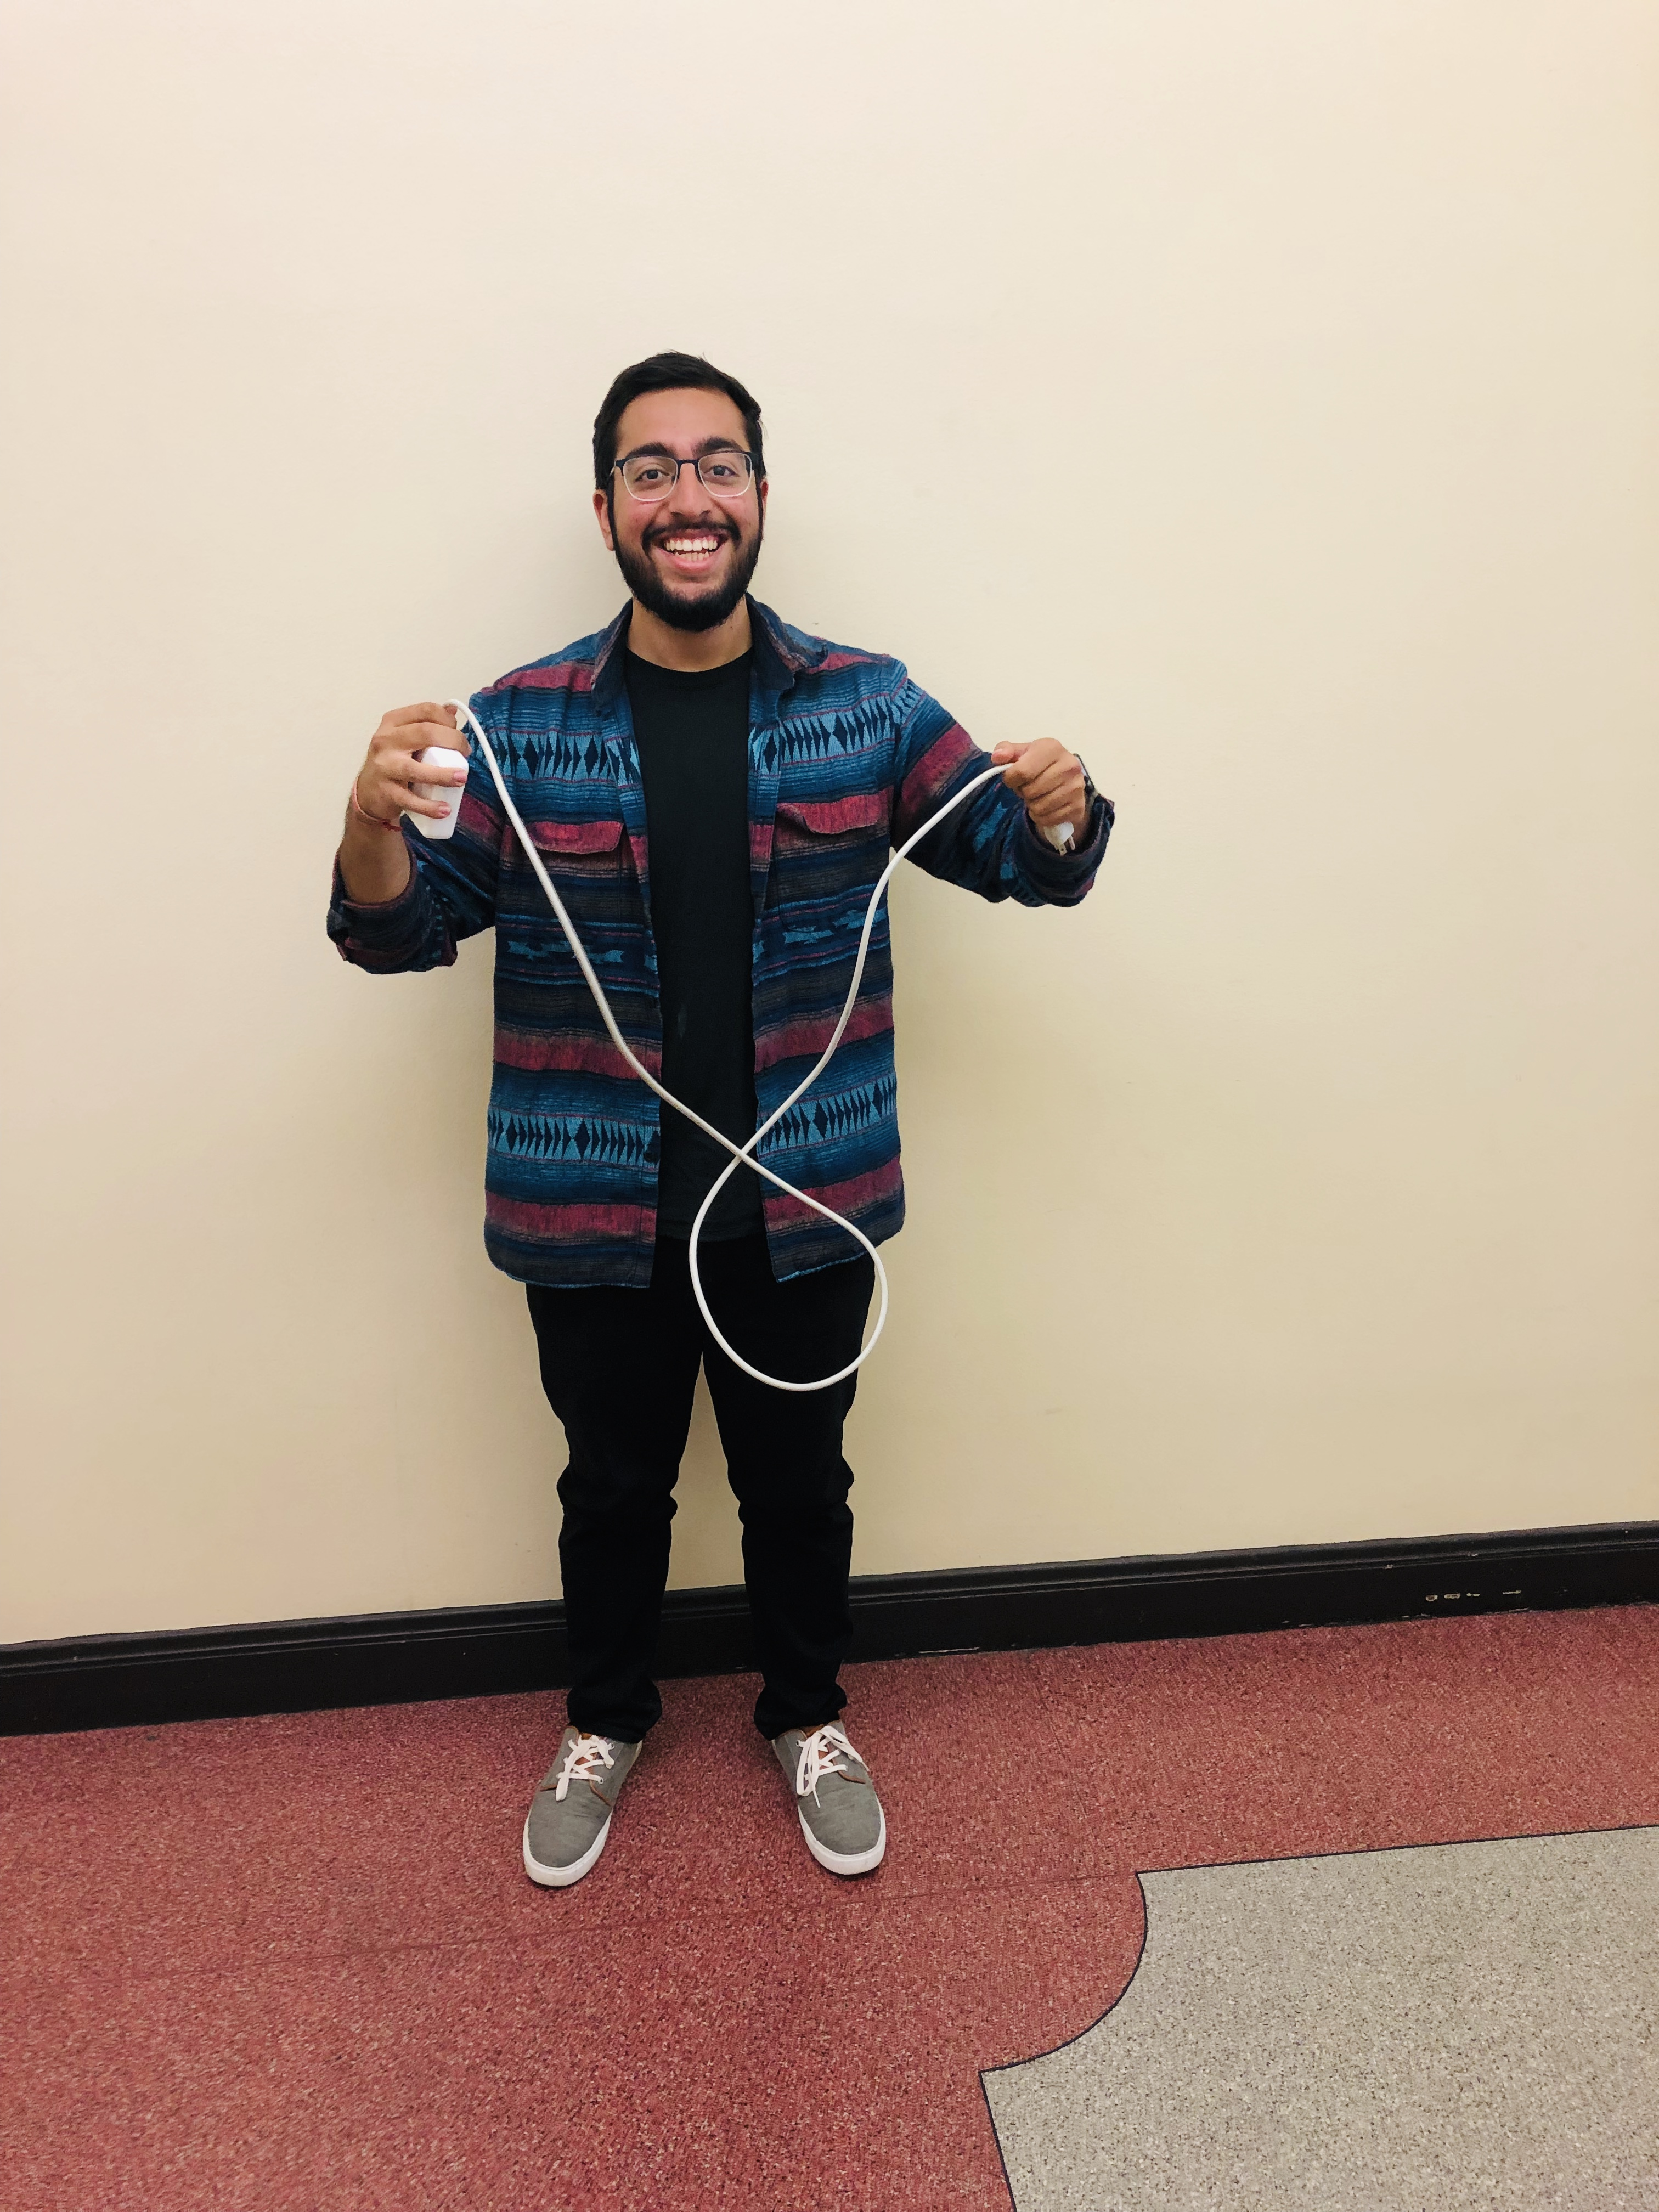
\includegraphics[height=9cm]{figures/sa.jpg}
    \caption{GSI Sukrit's laptop wire curve}
  \end{minipage}
\end{figure}
    \sol{
    \item
\[
g(x) = \begin{bmatrix}
x_1^2/x_2 \\
\log(x_3) \sin(x_1/x_3)
\end{bmatrix}
\]
    }

\end{enumerate}

\newpage
\qns{PSD equivalence: the Schur complement}\\ 
 Let $A \in \mathbb{S}^{n}$, $C \in \mathbb{S}^{m}$, $B \in \Real{n\times m}$, and consider the block matrix
 
 \[
 M = \begin{bmatrix}
A & B \\ 
B^T & C
\end{bmatrix}.
\]

\begin{enumerate}

\qitem Let $f(x, y) = \begin{bmatrix}
    x \\
    y
    \end{bmatrix}^\top M
    \begin{bmatrix}
    x \\
    y
    \end{bmatrix}$, for $x \in \R n$ and $y \in \R m$. Prove that for any $y$, if $A$ is positive definite, we have

\[
\min_x f(x, y) = y\tran (C- B^T A^{-1} B) y.
\]

\sol{\item $g(x_1,x_2) = \dfrac{x_1^2}{4} + \dfrac{x_2^2}{9}$


}

\qitem Prove that if $A$ is positive definite, then 
\[
S_A \doteq C- B^T A^{-1} B \succeq 0 \Longleftrightarrow  M = \begin{bmatrix}
A & B \\ 
B^T & C
\end{bmatrix} \succeq 0.
\]

\textit{Hint: $M$ is positive semi-definite if and only if 
\[
\min_{x,y} \begin{bmatrix}
x \\
y
\end{bmatrix}^\top M 
\begin{bmatrix}
x \\
y
\end{bmatrix} \geq 0
\]
}

\sol{\item Show that the following inequalities hold for any vector $x \in \Real{n}$:
\[
% \|x\|_\infty \le \|x\|_1 \le n \|x\|_\infty \\
% \|x\|_2 \le \|x\|_1 \le \sqrt{n} \|x\|_2 \\
% \|x\|_\infty \le \|x\|_2 \le\sqrt{n}\|x\|_\infty \\
\frac{1}{\sqrt{n}}\|x\|_2 \leq \|x\|_\infty \leq  \|x\|_2 \leq \|x\|_1 \leq \sqrt{n} \|x\|_2 \le n\|x\|_\infty.
\]

\textit{Hint:} For $\|x\|_1\leq \sqrt{n}\|x\|_2$, how might you express $\|x\|_1$ as the dot product of two vectors? Can you then use the Cauchy-Schwarz inequality to bound this dot product?}
\qitem Similarly, prove that if $C$ is positive definite, then
\[
S_C \doteq A - B C^{-1} B^T \succeq 0 \Longleftrightarrow  M = \begin{bmatrix}
A & B \\ 
B^T & C
\end{bmatrix} \succeq 0.
\]

\sol{\item $g(x) = \sin(x_1^2) \log (x_3 - x_2)$ where $x_i$ are scalars and $x_3 - x_2 > 0$.}

To go further, feel free to read:
\begin{itemize}
    \item \href{https://en.wikipedia.org/wiki/Schur_complement}{The wikipedia page of the Schur complement}
\end{itemize}


\end{enumerate}
\newpage
\qns{Catenary}

In this exercise, we will show that a string suspended on both side form a convex function (c.f. Figure \ref{fig:gsi}). 

\begin{figure}[h]
\centering
\includegraphics[width=.4\textwidth]{figures/catenary.png}
\caption{Happy GSI with his representation of convex function.}
\label{fig:gsi}
\end{figure}

More formally, this exercise wants to show that a \textbf{catenary} is a convex function. 
A catenary is the curve that an idealized hanging chain or cable assumes under its own weight when supported only at its ends (Wikipedia).

Catenaries are important shapes for buildings because the internal compression forces are ideally compensated (c.f. Figure \ref{fig:bridge}).
It is also a natural form in nature as the shape minimizes free energy (c.f. Figure \ref{fig:soap}).

\begin{figure}[h]
\centering
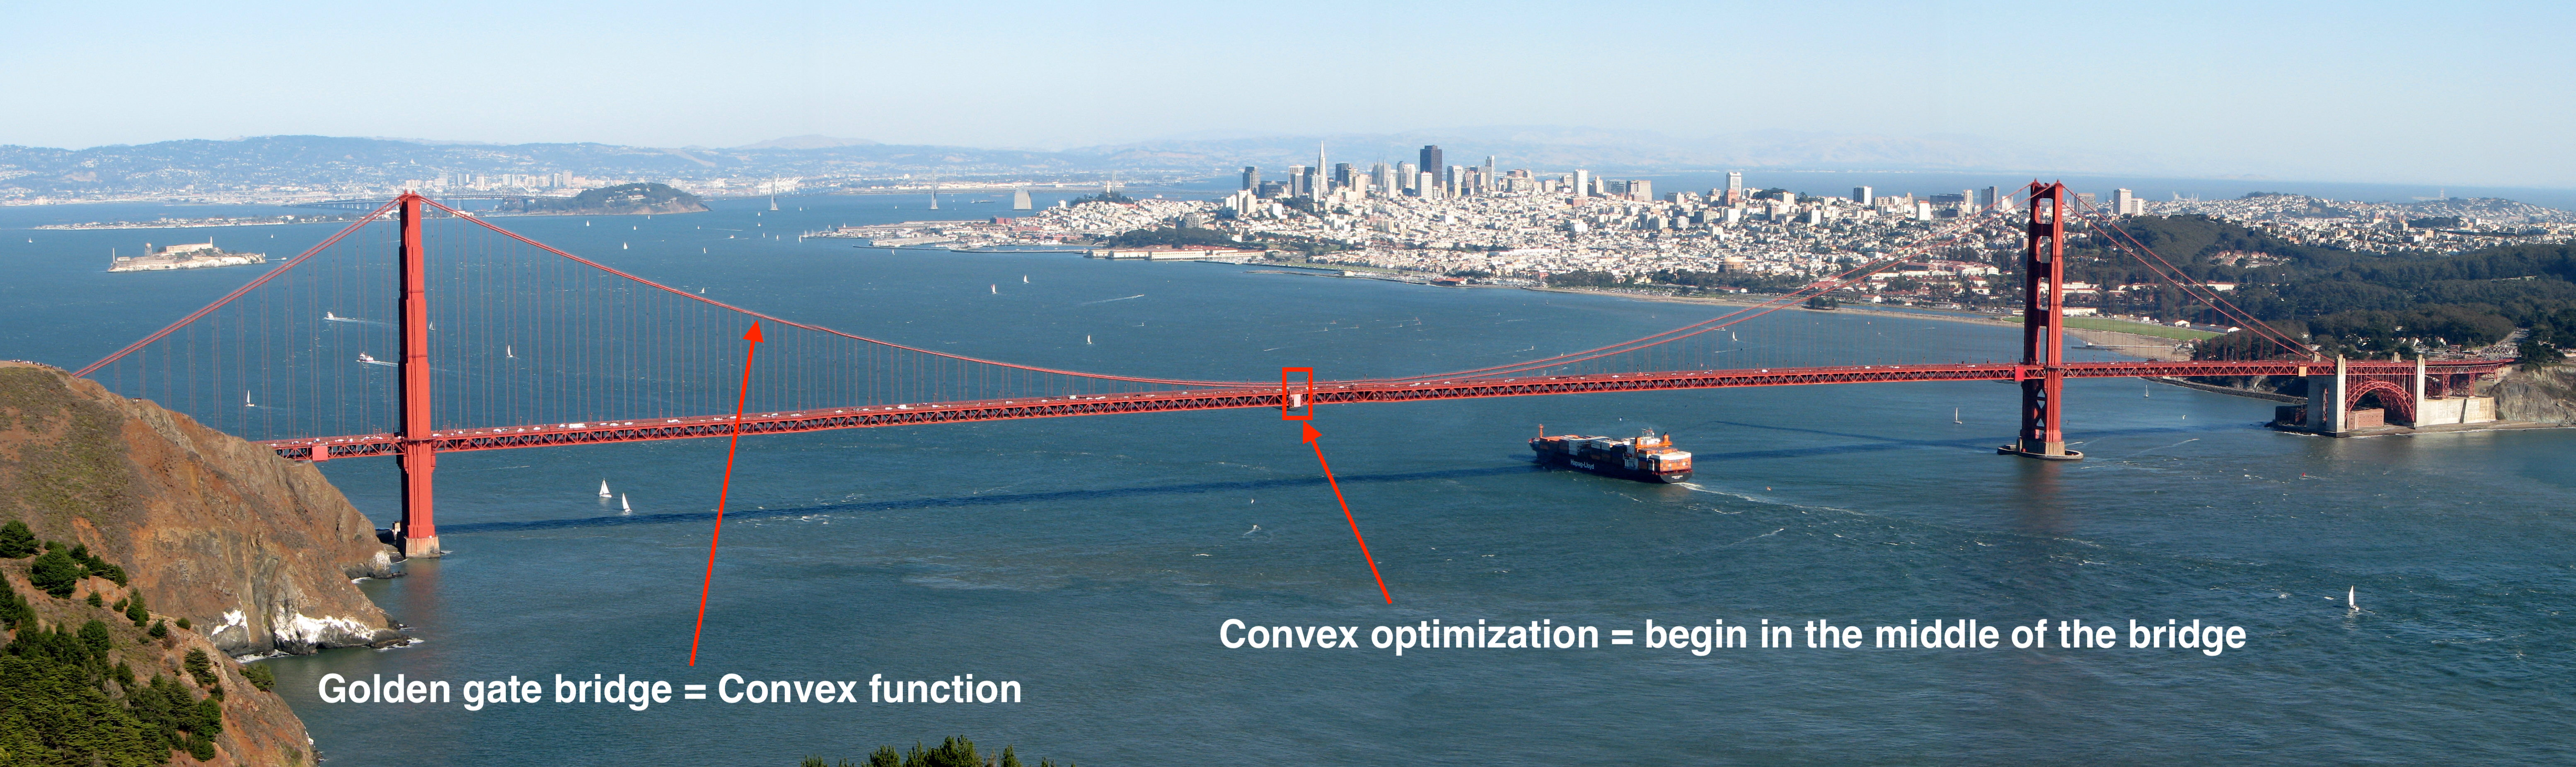
\includegraphics[width=.95\textwidth]{figures/golden_gate.jpg}
\caption{When you think about convex optimization, think about beginning in the middle of the Golden Gate Bridge!}
\label{fig:bridge}
\end{figure}

\begin{figure}[h]
\centering
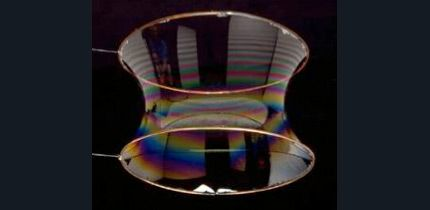
\includegraphics[width=.4\textwidth]{figures/soap.jpg}
\caption{Catenary is a shape that minimizes free energy, the vertical cut of soap film between two circles forms a catenary.}
\label{fig:soap}
\end{figure}

Let derive the equation for the catenary.
First, we need to introduce the notation (maybe the most difficult part of the exercise, see Figure \ref{fig:notations}):

\begin{figure}[h]
\centering
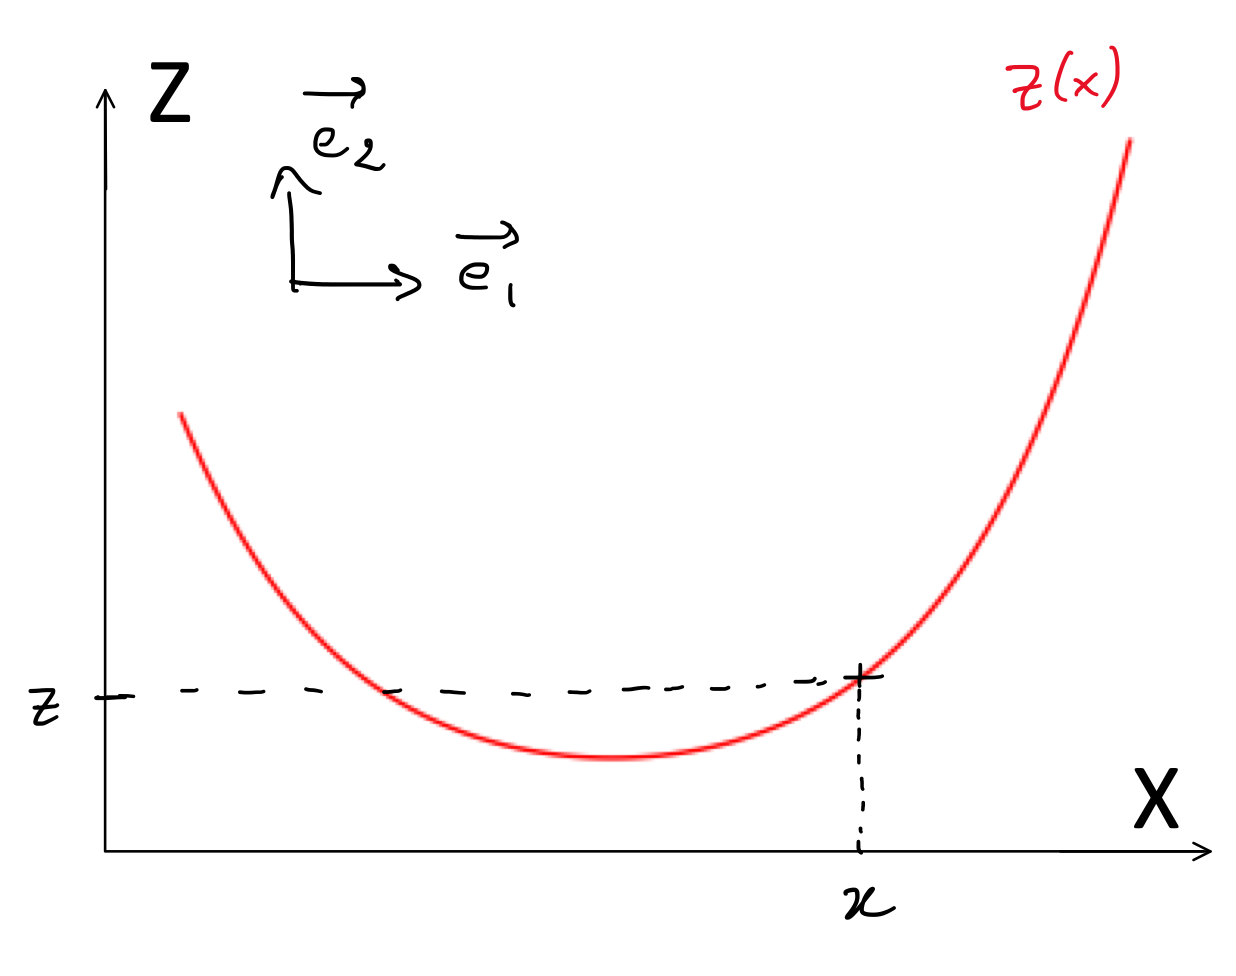
\includegraphics[width=.4\textwidth]{figures/graph.png}
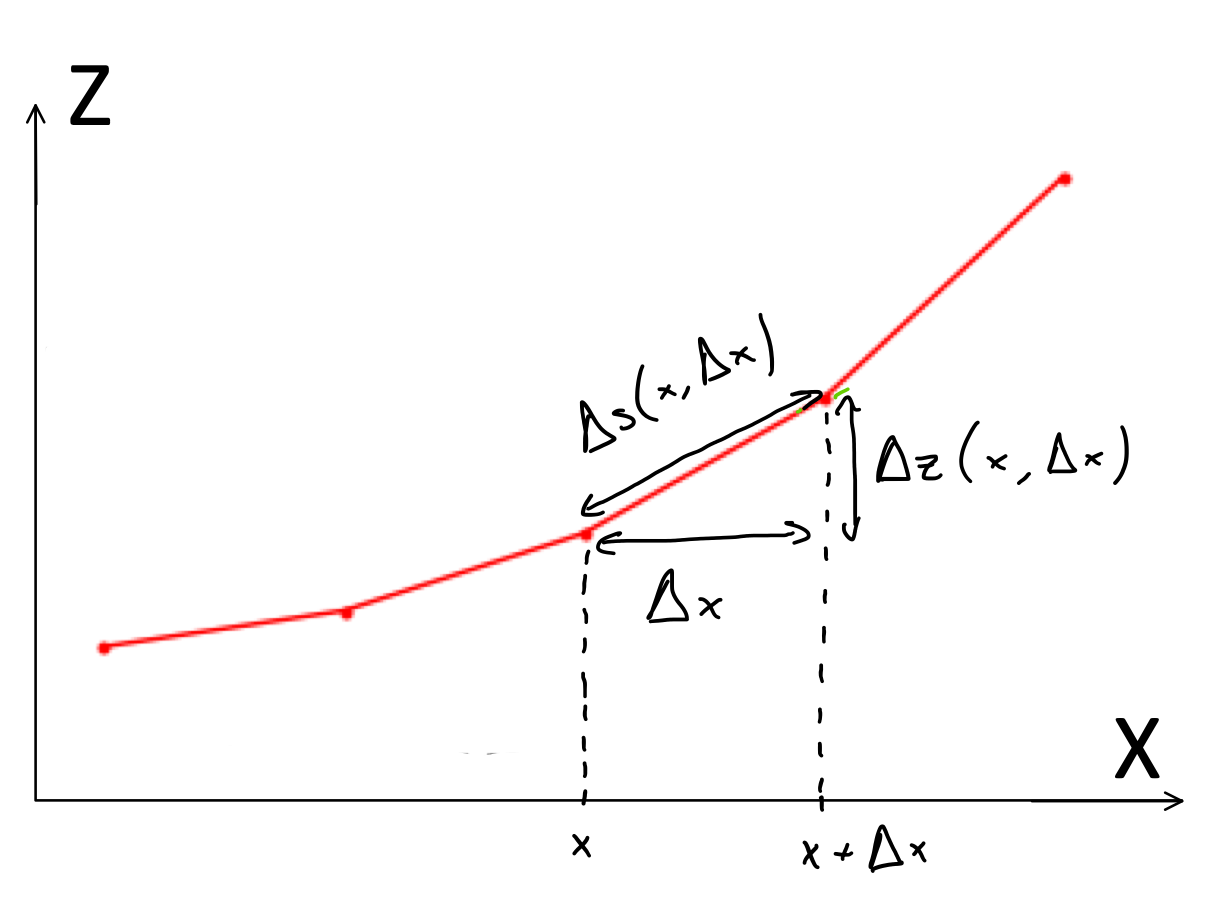
\includegraphics[width=.4\textwidth]{figures/length.png}

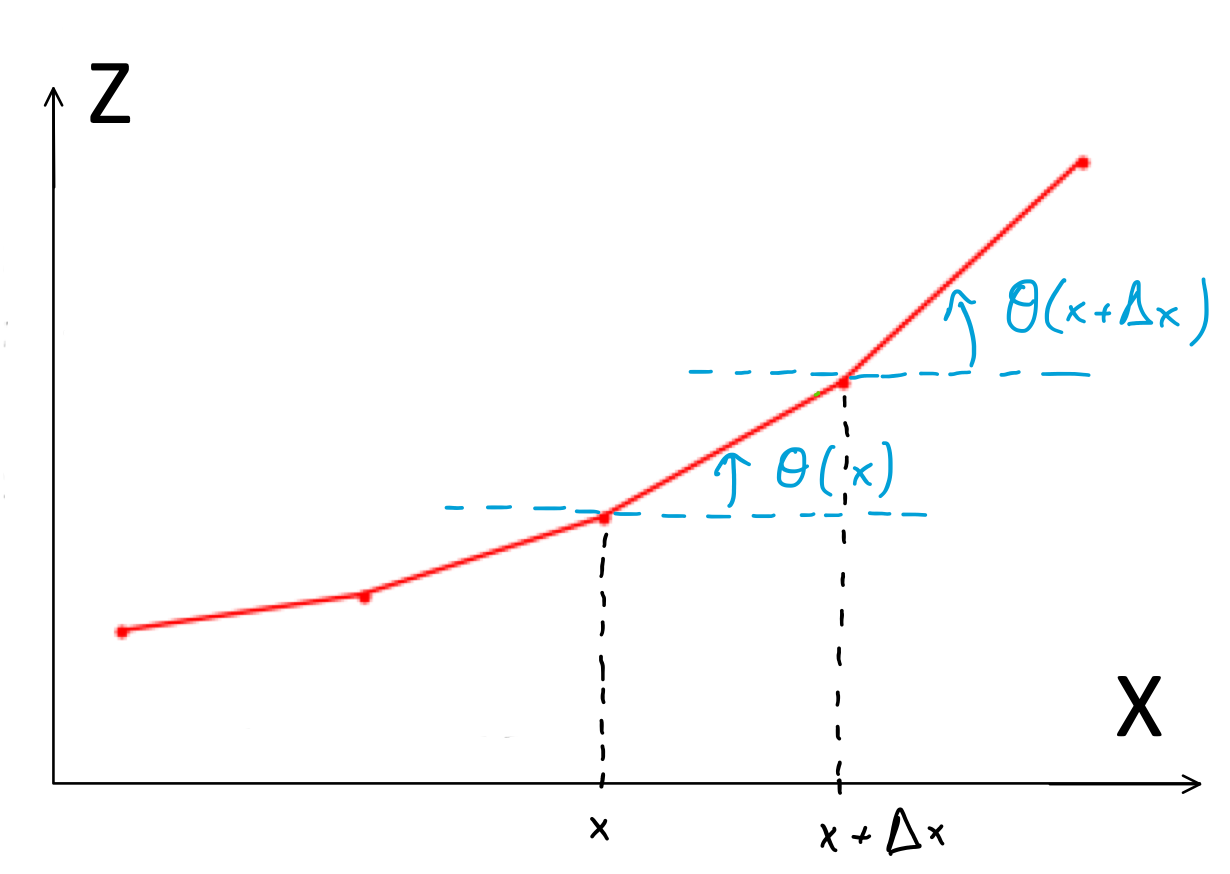
\includegraphics[width=.4\textwidth]{figures/angles.png}
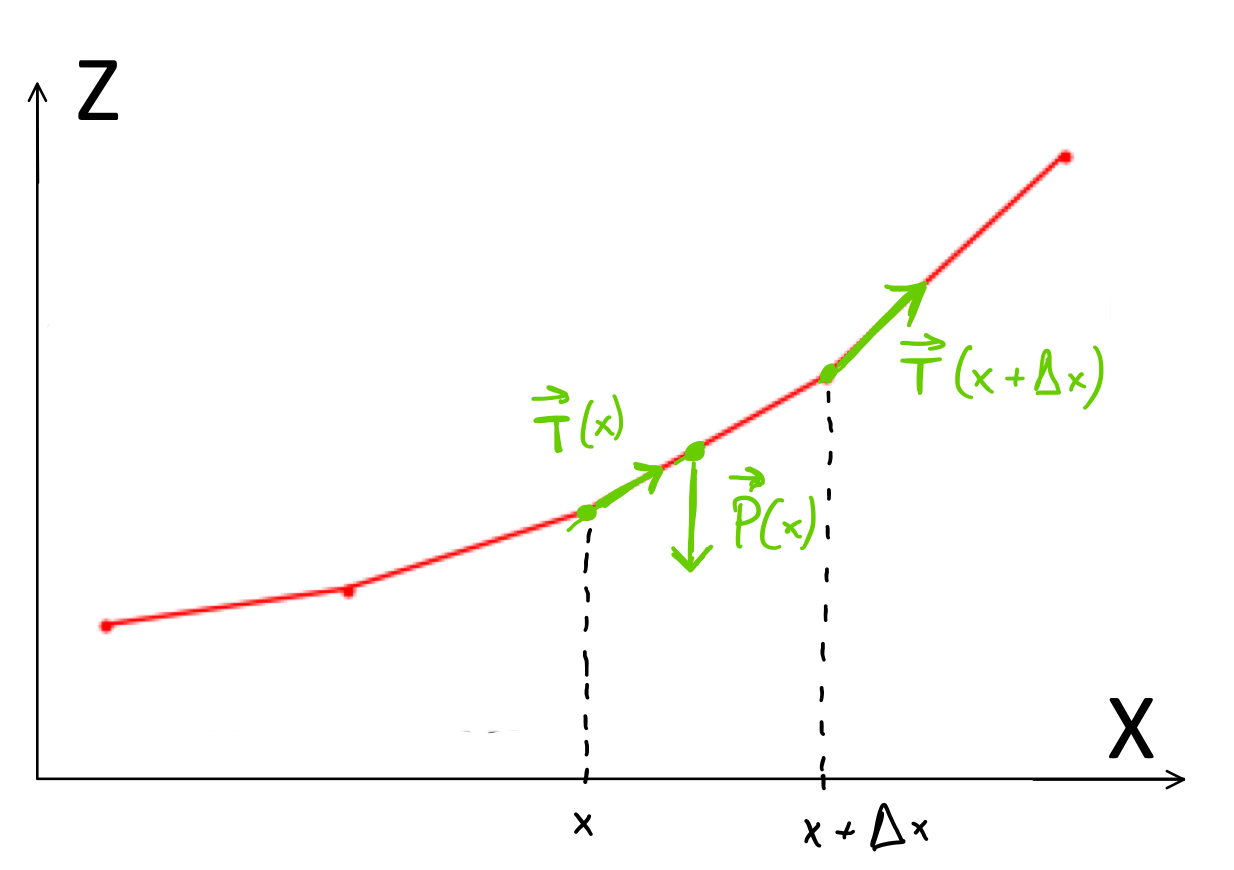
\includegraphics[width=.4\textwidth]{figures/forces.png}
\caption{Figures to help define the notation.}
\label{fig:notations}
\end{figure}

\begin{itemize}
    \item $x$ the horizontal coordinate.
    \item $z$ the vertical coordinate.
    \item $z(x)$ the equation of the catenary: we want to show that $z:x\mapsto z(x)$ is a convex function.
    \item $\Delta x$ the step for the approximation of the equation.
    \item $\Delta z(x,\Delta x) = z(x+\Delta x) - z(x)$ the vertical length at $x$ for a step size $\Delta x$.
    \item $\Delta s(x, \Delta x) = \sqrt{(\Delta x)^2 + (\Delta z(x,\Delta x))^2}$ the length of the chain between $x$ and $x+\Delta x$.
    \item $\theta(x)$ the angle between the horizontal axis and the string at $x$.
    \item $\overrightarrow{T}(x)$ the internal tension of the chain at $x$. More precisely, $\overrightarrow{T}(x)$ is the force on the segment of string to the right of $x$ due to the segment to the left of $x$.  We assume the string has no stiffness so $\overrightarrow{T}(x)$ is parallel to it, i.e.\ $\overrightarrow{T}(x) = T(x) \cos{\theta(x)} \overrightarrow{e_1} + T(x) \sin{\theta(x)} \overrightarrow{e_2}$.
    \item $\mu$ the linear density of the string.
    \item $g$ the acceleration of earth.
    \item $\overrightarrow{P}(x, \Delta x)$ the force of gravity. Physics gives us that $\overrightarrow{P}(x, \Delta x) = -\mu g \Delta s(x,\Delta x) \overrightarrow{e_2}$.
\end{itemize}

Since the string is static, the forces at each point must balance, i.e. $-\overrightarrow{T}(x)+\overrightarrow{T}(x+\Delta x)+ \overrightarrow{P}(x, \Delta x) = \overrightarrow{0}$.


\begin{enumerate}
    \qitem Show that the horizontal component of $\overrightarrow{T}(x)$ does not depend on $x$: show that $\exists T_0$ such that $\forall x,\ T(x)\cos{\theta (x)}=T_0$.
    
    \sol{\item $g(x_1,x_2) = \dfrac{x_1^2}{4} + \dfrac{x_2^2}{9}$


}
    \qitem Show that $-T(x)\sin{\theta (x)}+T(x+\Delta x)\sin{\theta (x+\Delta x)}=\mu g \Delta s(x,\Delta x)$.
    
    \sol{\item Show that the following inequalities hold for any vector $x \in \Real{n}$:
\[
% \|x\|_\infty \le \|x\|_1 \le n \|x\|_\infty \\
% \|x\|_2 \le \|x\|_1 \le \sqrt{n} \|x\|_2 \\
% \|x\|_\infty \le \|x\|_2 \le\sqrt{n}\|x\|_\infty \\
\frac{1}{\sqrt{n}}\|x\|_2 \leq \|x\|_\infty \leq  \|x\|_2 \leq \|x\|_1 \leq \sqrt{n} \|x\|_2 \le n\|x\|_\infty.
\]

\textit{Hint:} For $\|x\|_1\leq \sqrt{n}\|x\|_2$, how might you express $\|x\|_1$ as the dot product of two vectors? Can you then use the Cauchy-Schwarz inequality to bound this dot product?
    }
    \qitem Show that $- \tan{(\theta (x))} + \tan{(\theta (x+\Delta x))} = \frac{\mu g}{T_0} \Delta s(x,\Delta x)$.
    
    \sol{\item $g(x) = \sin(x_1^2) \log (x_3 - x_2)$ where $x_i$ are scalars and $x_3 - x_2 > 0$.
    }
    \qitem Show that $-\frac{\Delta z(x, \Delta x)}{\Delta x} + \frac{\Delta z(x+\Delta x, \Delta x)}{\Delta x} = \frac{\mu g}{T_0} \Delta s(x,\Delta x)$.
    
    \sol{\item
\[
g(x) = \begin{bmatrix}
x_1^2/x_2 \\
\log(x_3) \sin(x_1/x_3)
\end{bmatrix}
\]}
    
    \qitem Show that $\frac{\partial^2 z}{\partial x^2}(x) = \lim\limits_{\Delta x = 0} \frac{\mu g}{T_0} \frac{\Delta s(x,\Delta x)}{\Delta x}$.
    
    \sol{\input{catenary_solutions/5.tex}
    }
    
    \qitem Prove that $z:x\mapsto z(x)$ is a convex function.
    
    \sol{\input{catenary_solutions/6.tex}
    }
\end{enumerate}

Now we will go a little bit further in the exercise, and find the shape of the catenary explicitly.

\begin{enumerate}
    \setcounter{enumi}{6}
    \qitem Show that $\frac{\Delta s(x,\Delta x)}{\Delta x} = \sqrt{1+\left(\frac{\Delta z (x, \Delta x)}{\Delta x}\right)^2}$
    
    \sol{\input{catenary_solutions/7.tex}}
    \qitem As a first approximation, imagine that $\frac{\Delta z (x, \Delta x)}{\Delta x} \sim 0$. Show that $z(x) = ax^2+bx+c$. State the value of a.
    
    \sol{\input{catenary_solutions/8.tex}}
    \qitem Now, show that  $\frac{\partial^2 z}{\partial x^2}(x) = 
    \frac{\mu g}{T_0} \sqrt{1+\left(\frac{\partial z}{\partial x}(x)\right)^2}$.
    
    \sol{\input{catenary_solutions/9.tex}}
    
    \qitem Show that $z(x) = d\cdot \cosh{(\frac{x}{d})}$ is a solution. State the value of $d$. Compare it to the value of $a$ obtained in question (h).
    
    \sol{\input{catenary_solutions/10.tex}
    }
\end{enumerate}

\underline{Remark:} Notice that the curves of $z(x)=\frac{x^2}{2}$ and $z(x)=\cosh{(x)}-1$ are very similar around $x=0$. Indeed, $\cosh{(x)}-1 - \frac{x^2}{2} = O(x^4)$.

\underline{Remark:} Also notice that we have not shown that the solution is unique (even if this is the case).

To go further, feel free to read:
\begin{itemize}
    \item \href{https://en.wikipedia.org/wiki/Catenary}{The Wikipedia page of catenary}
    \item \href{https://www.math24.net/equation-catenary/}{The derivation of the equation of catenary on Math24.net}
\end{itemize}

\newpage
\qns{Solving a simple optimization problem using \texttt{cvxpy}}\\
In this problem we will solve a simple optimization problem using \texttt{cvxpy}. We have the following optimization problem:\\
\begin{align*}
    \text{minimize}\;\;\; 5x_0 + &6x_1 + 2x_2 + 9x_3\\
    \text{subject to,}\\
    x_0,x_1,x_2,x_3 &\geq 0\\
    2x_0 - 3x_1 &\leq 1\\
    x_0 + 3x_1 + 2x_3  &= 12\\
    2x_1 + 5x_2 &\geq 15\\
\end{align*}
\begin{enumerate}
    \item 
    Is the problem convex? Justify your answer.
    
    \sol{
    \item $g(x_1,x_2) = \dfrac{x_1^2}{4} + \dfrac{x_2^2}{9}$



    }
    \item
    Solve the problem using \texttt{cvxpy} in iPython notebook. Please refer to \url{https://www.cvxpy.org/tutorial/index.html} for more familiarity with \texttt{cvxpy}.
    
    \sol{
    \item Show that the following inequalities hold for any vector $x \in \Real{n}$:
\[
% \|x\|_\infty \le \|x\|_1 \le n \|x\|_\infty \\
% \|x\|_2 \le \|x\|_1 \le \sqrt{n} \|x\|_2 \\
% \|x\|_\infty \le \|x\|_2 \le\sqrt{n}\|x\|_\infty \\
\frac{1}{\sqrt{n}}\|x\|_2 \leq \|x\|_\infty \leq  \|x\|_2 \leq \|x\|_1 \leq \sqrt{n} \|x\|_2 \le n\|x\|_\infty.
\]

\textit{Hint:} For $\|x\|_1\leq \sqrt{n}\|x\|_2$, how might you express $\|x\|_1$ as the dot product of two vectors? Can you then use the Cauchy-Schwarz inequality to bound this dot product?
    }
\end{enumerate}


\newpage
\qns{Class survey}\\
Please, answer the following survey: \url{https://docs.google.com/forms/d/e/1FAIpQLSf-oF0H5l_nv3BrBxsT2MbjDwjRc95m46hZWMPHmsYEPfMt9Q/viewform?usp=sf_link}

Please submit to gradescope -- on the specific assignment for it -- a screen shot of the last page of the survey as a png file (with the text ``Thank you for your feedback on EECS 127/227A!'').

\end{qunlist}
\end{document}
